\documentclass[aspectratio=169,11pt]{beamer}

% ============================================================
% PACKAGES
% ============================================================
\usepackage{graphicx}
\usepackage{tikz}
\usetikzlibrary{positioning,arrows.meta}
\usepackage{xcolor}
\usepackage{booktabs}
\usepackage{tabularx}
\usepackage{array}
\usepackage{ragged2e}
\usepackage{hyperref}

% ============================================================
% COLORS - SAME AS PHASE-I
% ============================================================
\definecolor{GEUBlue}{RGB}{20,55,105}
\definecolor{GEULightBlue}{RGB}{238,244,251}
\definecolor{GEUGrey}{RGB}{90,90,90}
\definecolor{GEULightGrey}{RGB}{245,246,248}

% ============================================================
% BEAMER SETTINGS
% ============================================================
\usetheme{default}
\setbeamertemplate{navigation symbols}{}
\setbeamertemplate{blocks}[rounded][shadow=false]

\setbeamercolor{normal text}{fg=black,bg=white}
\setbeamercolor{frametitle}{fg=GEUBlue}
\setbeamercolor{structure}{fg=GEUBlue}
\setbeamercolor{block title}{fg=GEUBlue,bg=GEULightBlue}
\setbeamercolor{block body}{fg=black,bg=GEULightBlue}

\setbeamerfont{frametitle}{size=\Large,series=\bfseries}

% ============================================================
% LOGO
% ============================================================
% Upload Graphic Era logo as graphicera_logo.png
\newcommand{\GEULogo}{graphicera_logo.png}

% ============================================================
% HEADER
% ============================================================
\setbeamertemplate{headline}{%
  \begin{tikzpicture}[remember picture,overlay]
    \node[
        anchor=north east,
        xshift=-0.30cm,
        yshift=-0.12cm
    ] at (current page.north east)
    {\includegraphics[height=0.62cm]{\GEULogo}};
  \end{tikzpicture}
  \vspace{0.72cm}
}

% ============================================================
% FRAME TITLE
% ============================================================
\setbeamertemplate{frametitle}{%
  \vspace{0.03cm}
  \insertframetitle\par
  \vspace{0.04cm}
  \textcolor{GEUBlue}{\rule{\textwidth}{0.9pt}}
  \vspace{0.03cm}
}

% ============================================================
% FOOTER
% ============================================================
\setbeamertemplate{footline}{%
  \leavevmode
  \hbox{%
  \begin{beamercolorbox}[
      wd=.82\paperwidth,
      ht=0.32cm,
      dp=0.10cm,
      leftskip=.3cm
  ]{author in head/foot}
    
  \end{beamercolorbox}%
  \begin{beamercolorbox}[
      wd=.18\paperwidth,
      ht=0.32cm,
      dp=0.10cm,
      rightskip=.3cm
  ]{date in head/foot}
    \hfill\tiny\insertframenumber/\inserttotalframenumber
  \end{beamercolorbox}}
}

% ============================================================
% CUSTOM COMMANDS
% ============================================================
\newcommand{\smallnote}[1]{%
\vspace{0.08cm}
{\scriptsize\color{GEUGrey}#1}
}

\newcommand{\placeholder}[1]{%
\textit{\color{GEUGrey}#1}
}

% ============================================================
% DOCUMENT INFORMATION
% ============================================================
\title{\textbf{Project-Based Learning}\\[2mm]\large Phase-III Evaluation}

\author{
\textbf{PrioriTask:Intelligent Task Scheduling System}\\
Team ID: T-315
}

\institute{
Department of Computer Science \& Engineering\\
Graphic Era (Deemed to be University), Dehradun
}

\date{Academic Session 2026--27}

% ============================================================
% DOCUMENT
% ============================================================
\begin{document}

% ============================================================
% SLIDE 1
% ============================================================
\begin{frame}[plain]

\begin{tikzpicture}[remember picture,overlay]

\draw[GEUBlue,line width=3pt]
(current page.north west) -- (current page.north east);

\node[
    anchor=north east,
    xshift=-0.45cm,
    yshift=-0.35cm
] at (current page.north east)
{\includegraphics[height=1.0cm]{\GEULogo}};

\node[
    align=center,
    text width=.84\paperwidth
] at ([yshift=.25cm]current page.center)
{
{\color{GEUBlue}
\fontsize{26}{30}\selectfont
\bfseries PROJECT-BASED LEARNING}
\\[3mm]

{\fontsize{18}{22}\selectfont
PHASE-III FINAL EVALUATION}
\\[7mm]

{\color{GEUGrey}
\Large\bfseries
PrioriTask:Intelligent Task Scheduling System}
\\[3mm]

{\color{GEUBlue}
\normalsize Team ID: T-315}
};

\node[
    align=center,
    anchor=south,
    yshift=.42cm
] at (current page.south)
{
\bfseries
Department of Computer Science \& Engineering\\
Graphic Era (Deemed to be University), Dehradun\\[-1mm]
\scriptsize Academic Session 2026--27
};

\end{tikzpicture}

\end{frame}

% ============================================================
% SLIDE 2
% ============================================================
\begin{frame}{Team \& Mentor Details}

\begin{columns}[T,totalwidth=\textwidth]

\column{.48\textwidth}

\begin{block}{Team Information}
\begin{tabular}{@{}ll@{}}
\textbf{Team ID:} & T-315\\
\textbf{Semester:} & 3rd\\
\textbf{Section:} & A, ML4, CYBER\\
\textbf{Domain:} & CSE
\end{tabular}
\end{block}

\column{.48\textwidth}

\begin{block}{Team Members}
1.\quad Manisha Bisht -- 2510012646\\
2.\quad Purnima -- 2510012541\\
3.\quad Yug Bhardwaj -- 2512500006
\end{block}

\end{columns}

\vspace{2mm}

\begin{block}{Mentor}
Dr. Hriday Kumar Gupta
\hfill
\textbf{Interactions:3} 
\end{block}

\vfill

\smallnote{

}

\end{frame}

% ============================================================
% SLIDE 3
% ============================================================
\begin{frame}{Project Abstract \& Problem Statement}

\begin{block}{Project Abstract}
A C++ and SQLite app that shrinks, drops and suggests tasks to fit an overbooked day.
\end{block}


\begin{block}{Problem Statement}
To-do apps sort tasks; PrioriTask decides how much of each task fits when the day is full.
\end{block}

\vspace{2mm}

\textbf{\color{GEUBlue}Target Users / Application}

\begin{itemize}\itemsep2pt
    \item Students and staff with fixed hours
    \item Offline desktop app: a realistic plan, fewer missed deadlines
\end{itemize}

\smallnote{

}

\end{frame}

% ============================================================
% SLIDE 4
% ============================================================
\begin{frame}{Objectives \& Final Deliverables}

\begin{columns}[T,totalwidth=\textwidth]

\column{.48\textwidth}

\textbf{\color{GEUBlue}Finalized Objectives}

\begin{enumerate}\itemsep3pt
    \item Ideal and minimum time per task
    \item Fit the day with two policies
    \item Drop optional tasks only if needed
    \item Suggest tasks by deadline,energy
    \item Track missed tasks every month
\end{enumerate}

\column{.48\textwidth}

\textbf{\color{GEUBlue}Final Deliverables}

\begin{itemize}\itemsep3pt
    \item Desktop GUI and 11-option CLI
    \item C++17 source code on GitHub
    \item SQLite database, 4 tables
    \item Phase-I, II and III reports
    \item Own DSA library and tests
\end{itemize}

\end{columns}

\vfill


\end{frame}

% ============================================================
% SLIDE 5
% ============================================================
\begin{frame}{Phase-I \& Phase-II Feedback Incorporated}

\scriptsize

\begin{center}

\renewcommand{\arraystretch}{1.35}

\begin{tabularx}{.96\textwidth}
{@{}p{2.1cm}X X@{}}

\toprule
\textbf{Phase} &
\textbf{Feedback / Suggestion} &
\textbf{Action Taken}\\
\midrule

Phase-I &
Correct implementation of C++ classes &
\texttt{Database} class owns the SQLite connection\\

Phase-I &
Extend the core idea of the project &
Added dropping, advisor, commitments, dashboard\\

Phase-I &
Scheduler output overwrote task definitions &
Separate \texttt{day\_plan} table per day\\

Phase-II &
GUI headers should be in the project &
Dear ImGui added to \texttt{third\_party/}\\


\bottomrule

\end{tabularx}

\end{center}

\vfill

\begin{block}{Final Improvement}
From a compression engine to a full desktop app with dropping, advice and a dashboard.
\end{block}

\smallnote{

}

\end{frame}

% ============================================================
% SLIDE 6
% ============================================================
\begin{frame}{Final System Architecture}

\begin{center}

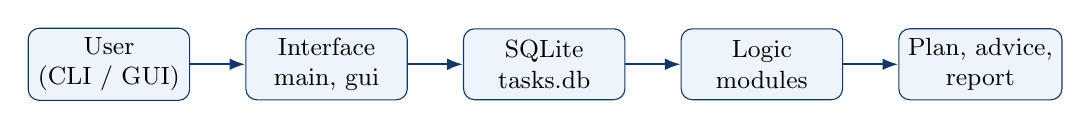
\begin{tikzpicture}[
node distance=7mm,
box/.style={
rectangle,
rounded corners,
draw=GEUBlue,
fill=GEULightBlue,
minimum width=2.05cm,
minimum height=9mm,
align=center,
font=\small
},
arrow/.style={
-{Latex[length=2mm]},
thick,
draw=GEUBlue
}
]

\node[box] (a) {User\\(CLI / GUI)};
\node[box,right=of a] (b) {Interface\\main, gui};
\node[box,right=of b] (c) {SQLite\\tasks.db};
\node[box,right=of c] (d) {Logic\\modules};
\node[box,right=of d] (e) {Plan, advice,\\report};

\draw[arrow] (a)--(b);
\draw[arrow] (b)--(c);
\draw[arrow] (c)--(d);
\draw[arrow] (d)--(e);

\end{tikzpicture}

\end{center}

\vspace{4mm}

\begin{columns}[T,totalwidth=\textwidth]

\column{.48\textwidth}

\textbf{\color{GEUBlue}Major Components}

\begin{itemize}\itemsep2pt
    \item \texttt{database.h}: 4-table database
    \item Scheduler, advisor, monthly report
    \item \texttt{dsa.h}: own array, heap, sort
    \item CLI and Dear ImGui desktop GUI
\end{itemize}

\column{.48\textwidth}

\textbf{\color{GEUBlue}System Flow}

\begin{itemize}\itemsep2pt
    \item Tasks, commitments, energy
    \item Shrink, drop, score, merge
    \item \texttt{tasks.db}, saved in transactions
    \item Plan, suggestions, monthly report
\end{itemize}

\end{columns}

\vfill

\smallnote{
Brief Discussion: The logic never touches SQLite, so each algorithm is tested alone.
}

\end{frame}


% ============================================================
% SLIDE 7
% ============================================================
\begin{frame}{Final Technology Stack}

\begin{columns}[T,totalwidth=\textwidth]

\column{.48\textwidth}

\begin{block}{Software / Technologies}
\begin{itemize}\itemsep2pt
    \item Programming: C++17
    \item Framework: Dear ImGui 1.91.6
    \item Database: SQLite (compiled in)
    \item Libraries/APIs: GLFW, OpenGL 3
    \item OS/Platform: Windows 11, Ubuntu (WSL)
\end{itemize}
\end{block}

\column{.48\textwidth}

\begin{block}{Development Infrastructure}
\begin{itemize}\itemsep2pt
    \item IDE: VS Code
    \item Version Control: Git/GitHub
    \item Testing Tools: own C++ test programs
    \item Deployment: local desktop app
    \item Other Tools: g++ 15.2, DB Browser
\end{itemize}
\end{block}

\end{columns}

\vfill

\smallnote{
Brief Discussion: Builds moved from MinGW to Ubuntu (WSL) after antivirus blocked Windows builds.
}

\end{frame}

% ============================================================
% SLIDE 8
% ============================================================
\begin{frame}{Implementation of PBL Course Concepts}

\scriptsize

\begin{center}

\renewcommand{\arraystretch}{1.25}

\begin{tabularx}{.96\textwidth}
{@{}>{\bfseries}p{2.8cm}X p{2.8cm}@{}}

\toprule
Course & Concepts Actually Implemented & Project Module\\
\midrule

Data Structures in C &
Own dynamic array, binary heap (priority queue) and merge sort; no STL &
\texttt{dsa.h}, Scheduler\\

OOPs with C++ &
Classes, encapsulation, destructor (RAII), class templates, operator overloading &
Database, \texttt{dsa.h}\\

\midrule

Design \& Analysis of Algorithms &
Greedy task-dropping with a heap; interval merging; $O(n \log n)$ &
Scheduler, Commitments\\

DBMS &
Four tables; keys, CHECK, UNIQUE; transactions; GROUP BY &
Database\\

\bottomrule

\end{tabularx}

\end{center}

\vfill

\begin{center}
\colorbox{GEULightBlue}{
\parbox{.88\textwidth}{
\centering
\textbf{Stated honestly:}
only concepts present in the code are listed; each can be shown in its source file.
}}
\end{center}

\smallnote{
Brief Discussion: Our PBL courses are Data Structures and OOPs with C++; DAA and DBMS show further work.
}

\end{frame}

% ============================================================
% SLIDE 9
% ============================================================
\begin{frame}{Module-Wise Final Implementation}

\scriptsize

\begin{center}

\renewcommand{\arraystretch}{1.35}

\begin{tabularx}{.96\textwidth}
{@{}p{2.4cm}X p{2.0cm}p{2.0cm}@{}}

\toprule
\textbf{Module} &
\textbf{Implementation} &
\textbf{Responsible} &
\textbf{Status}\\
\midrule

Database &
4 tables, transactions, migration &
Purnima &
Completed\\

Compression, advisor &
Two shrink policies; task scoring, quiet mode &
Manisha &
Completed\\

Task-dropping &
Heap-based greedy drop, restore pass &
Yug &
Completed\\

Commitments, dashboard &
Busy-time merging; monthly on-time report &
Purnima &
Completed\\

CLI and GUI &
11-option menu, 5-tab desktop app &
Manisha &
Completed\\

DSA library &
Own array, heap and merge sort &
Yug &
Completed\\

\bottomrule

\end{tabularx}

\end{center}

\vspace{4mm}

\begin{center}
\colorbox{GEULightBlue}{
\parbox{.40\textwidth}{
\centering
\textbf{Final Project Completion:}
 100\% 
}}
\end{center}

\vfill

\smallnote{

}

\end{frame}

% ============================================================
% SLIDE 10
% ============================================================
\begin{frame}{Working System / Prototype Demonstration}

\begin{columns}[T,totalwidth=\textwidth]

\column{.43\textwidth}

\textbf{\color{GEUBlue}Major Working Features}

\begin{itemize}\itemsep3pt
    \item What now: best task, with reasons
    \item Plan my day: shrink, then drop
    \item Quiet mode in college; free slots
    \item Tasks and weekly commitments
    \item This month: on-time rate
\end{itemize}

\column{.53\textwidth}

\begin{block}{System Screenshot / Output}

\centering
\vspace{11mm}

\includegraphics[width=\linewidth,height=1.9cm,keepaspectratio]{planday.png}

\vspace{11mm}

\end{block}

\end{columns}

\vfill

\smallnote{
Brief Discussion: Live demo -- add a task, plan the day, check This month.
}

\end{frame}
